\subsection{Chirps during dyadic competitions}

We used our algorithm to detect chirps in a dyadic competition experiment where two individuals competed for one superior shelter. In this exemplary recording almost all physical contacts, chasing events, and chirps happened during the dark phase of the experiment (Figure \ref{fig:timeline}, top rows in raster plot). We can estimate that the winner (yellow) did not chirp as much as the loser (red) of the competition. In this example, the winner emitted only 10 chirps whereas the loser produced close to 400 chirps(Figure \ref{fig:timeline}).
\begin{figure}[H]
    \centering
    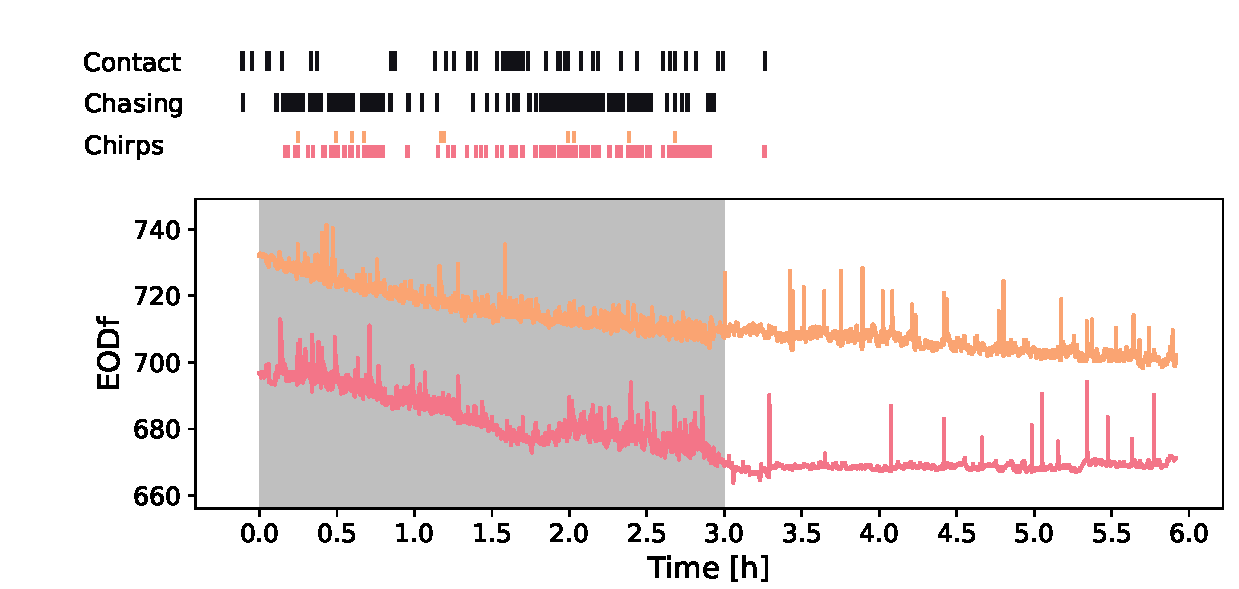
\includegraphics[width=\linewidth]{figures/timeline.pdf}
    \mycaption{Overview of a single trial of the competition experiment.}{The raster plots indicate the occurrence of the type of event. Rasterplots of chirps are color-coded with respect to the emitter of the chirp. The line plots indicate the EOD$f$ of the two fish over time as it was tracked on a spectrogram. Red was the winner of the competition, and yellow was the loser. The shaded area indicates the phase where lights were turned off.}
    \label{fig:timeline}
\end{figure}

Losers tended to chirp more than winners (Figure \ref{fig:winnerloser} A). This could be observed in 16 of the 22 valid trials (total n = 28) however this difference was not significant (Wilcoxon-test: z-statistic=67.0, pvalue=0.054). The outcome of the competition experiment was influenced by the size of the individuals. The winner of the dyadic interaction tended to have a greater size than the losers (Figure \ref{fig:winnerloser} B). For small size differences, there was an increase in chirp count, indicating that chirps increased in relevance for competition as the size difference decreased. The frequencies of the emitted EOD for winner and loser did not show any relevance for the outcome of the competition because the distribution for winner and loser is evenly spread over the range of EOD$f$ (Figure \ref{fig:winnerloser} C). 

\begin{figure}[H]
    \centering
    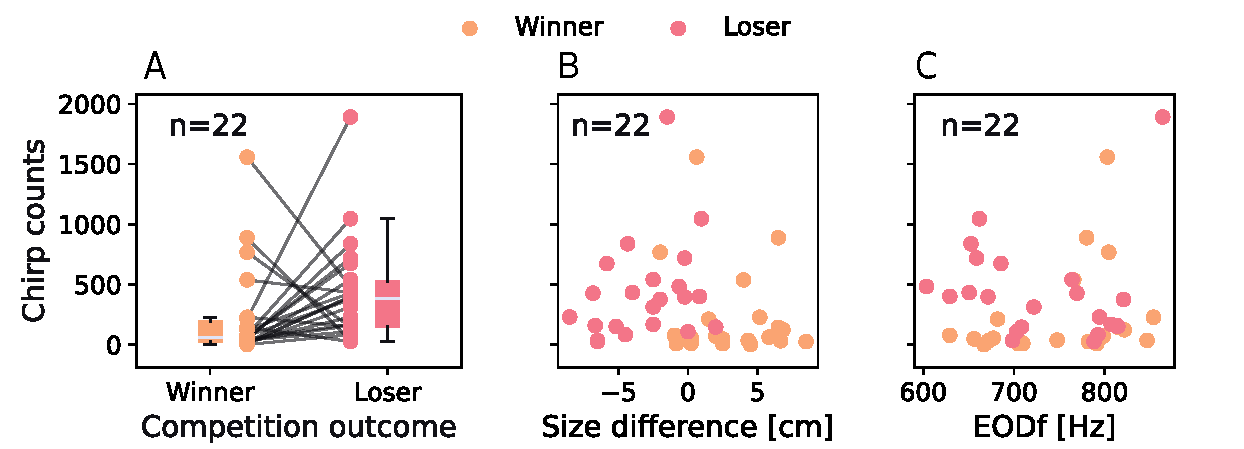
\includegraphics[width=\linewidth]{figures/chirps_winner_loser.pdf}
    \mycaption{Competition outcome }{compared to the emitted chirps in 22 valid parings (total n=28). \textbf{A:} Winner and loser of the competition experiment displayed with their quantity of chirps. Connecting lines indicate the pairing in the experiment. \textbf{B:} Winner and Loser compared to their size difference [cm] and the number of chirps they emitted. Losers (orange) are usually smaller than winners ($\Delta$ size $<$ 0) \textbf{C}: EOD$f$s [Hz] of the winner and loser compared to their quantity of chirps.}
    \label{fig:winnerloser}
\end{figure}

\subsection{Chirps emitted by loser fish might disrupt chasing events}

\begin{wrapfigure}{R}{0.6\textwidth}
\vspace{-1cm}
  \begin{center}
    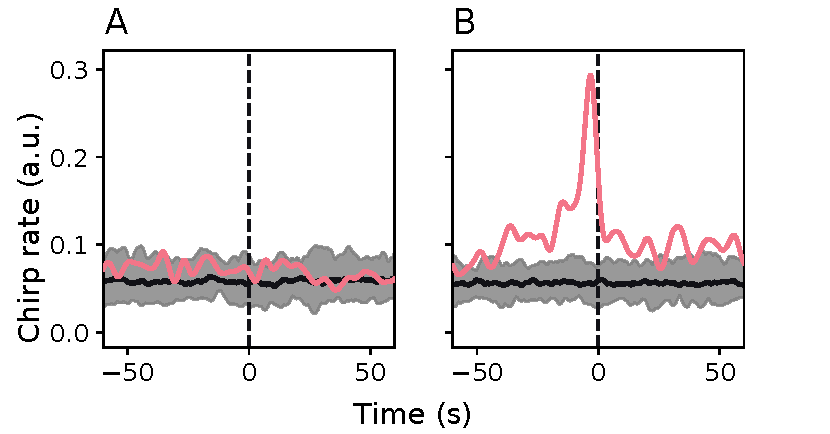
\includegraphics[width=\linewidth]{figures/kde.pdf}
    \end{center}
    \mycaption{Chasing-triggered chirps}{for two selected dyads. The time axis is centered around the offset of a chasing event. The black line indicates the bootstrapped baseline. The gray area is the bootstrapped confidence interval. The red line indicates the chirp rate estimated by a convolution with a Gaussian kernel. \textbf{A:} In most cases, there was no change in the chirp rate around an offset of a chasing event. \textbf{B:} But in a subset of the dataset chirping increased just before the chasing stopped.}
    \label{fig:kde}
\end{wrapfigure}

Losers tending to chirp more often than winners already hints towards a behavioral significance to chirps during competitions. We evaluated the temporal correlation of chirps and agnostic behaviors to further investigate the behavioral significance of chirps in dyadic encounters. For this, we computed the chasing-triggered chirp rate of the on- and offset of chasing events and contacts. The chasing-triggered chirp rate consists of chirps centered around agonistic events. After this sorting, we estimated the distribution of chirps for the events using a convolution with a Gaussian kernel. We focused on the offset of chasing events because the onset and physical contact did not show consistent increases in chirp rate. For approximately a third of all dyadic competitions, there was an increase in chirp rate before the offset occurred (Figure \ref{fig:kde} right). In the other cases, there was no interaction of the offset and chirps (Figure \ref{fig:kde} left). This was compared to a permutated baseline to show a significant increase in chirp rate. The summarized chirp rates across all competitions did not show an increase in chirp rate around the offsets of the chasing events.

\newpage
\FloatBarrier
\begin{wrapfigure}[14]{hr}{0.4\textwidth}
    \centering
    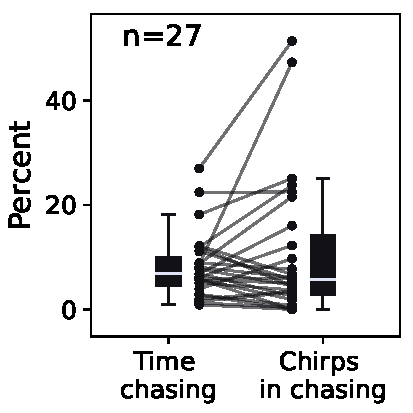
\includegraphics[width=\linewidth]{figures/chirps_in_chasing.pdf}
    \mycaption{Proportion of time spent and chirps emitted in chasing events.}{Relative time spent of the dark recording phase (3 h) in chasing events for single trials (\textbf{left}) and the relative quantity of chirps that were emitted during a chasing event for each recording (\textbf{right}). The lines show that the proportion of chirps during chasing events was only elevated for a subset of the competitions.}
    \label{fig:chasing}
\end{wrapfigure}
\FloatBarrier

To summarize this, we compared the percentage of time spent in chasing events with the percentage of chirps emitted in chasing events. This comparison should indicate that when the two fish are in a chasing event, and the chirps are used to carry information specifically related to competition, there should be an increase in the percentage of chirps in these chasing events. In 15 out of 27 pairings the percentage of time spent in chasing events was higher than the percentage of chirps emitted during chasing, showing that chirps may not be used for transferring information about their physical status in those cases. This indicates that chirps are not specifically used for the offset of chasing events because their percentage of occurrences is often lower than the time spent in these chasing events. 
